\section{Method}
\label{sec:method}

Given two textured 3D assets $S_1$ and $S_2$, our objective is to generate
a continuous morphing sequence controlled by an interpolation coefficient
$\alpha\in[0,1]$, with $\alpha=1$ corresponding to $S_1$ and $\alpha=0$
to $S_2$. We approach this task through a teacher--student framework
that transforms training-free morphing predictions into supervision for
a learnable generative model. By training on morphs produced from many different objects, the student learns a shared morphing function, rather than relying on a fixed interpolation procedure.
An overview of the proposed framework is shown in
Fig.~\ref{fig:architecture}.

\begin{figure*}[t]
 \centering
 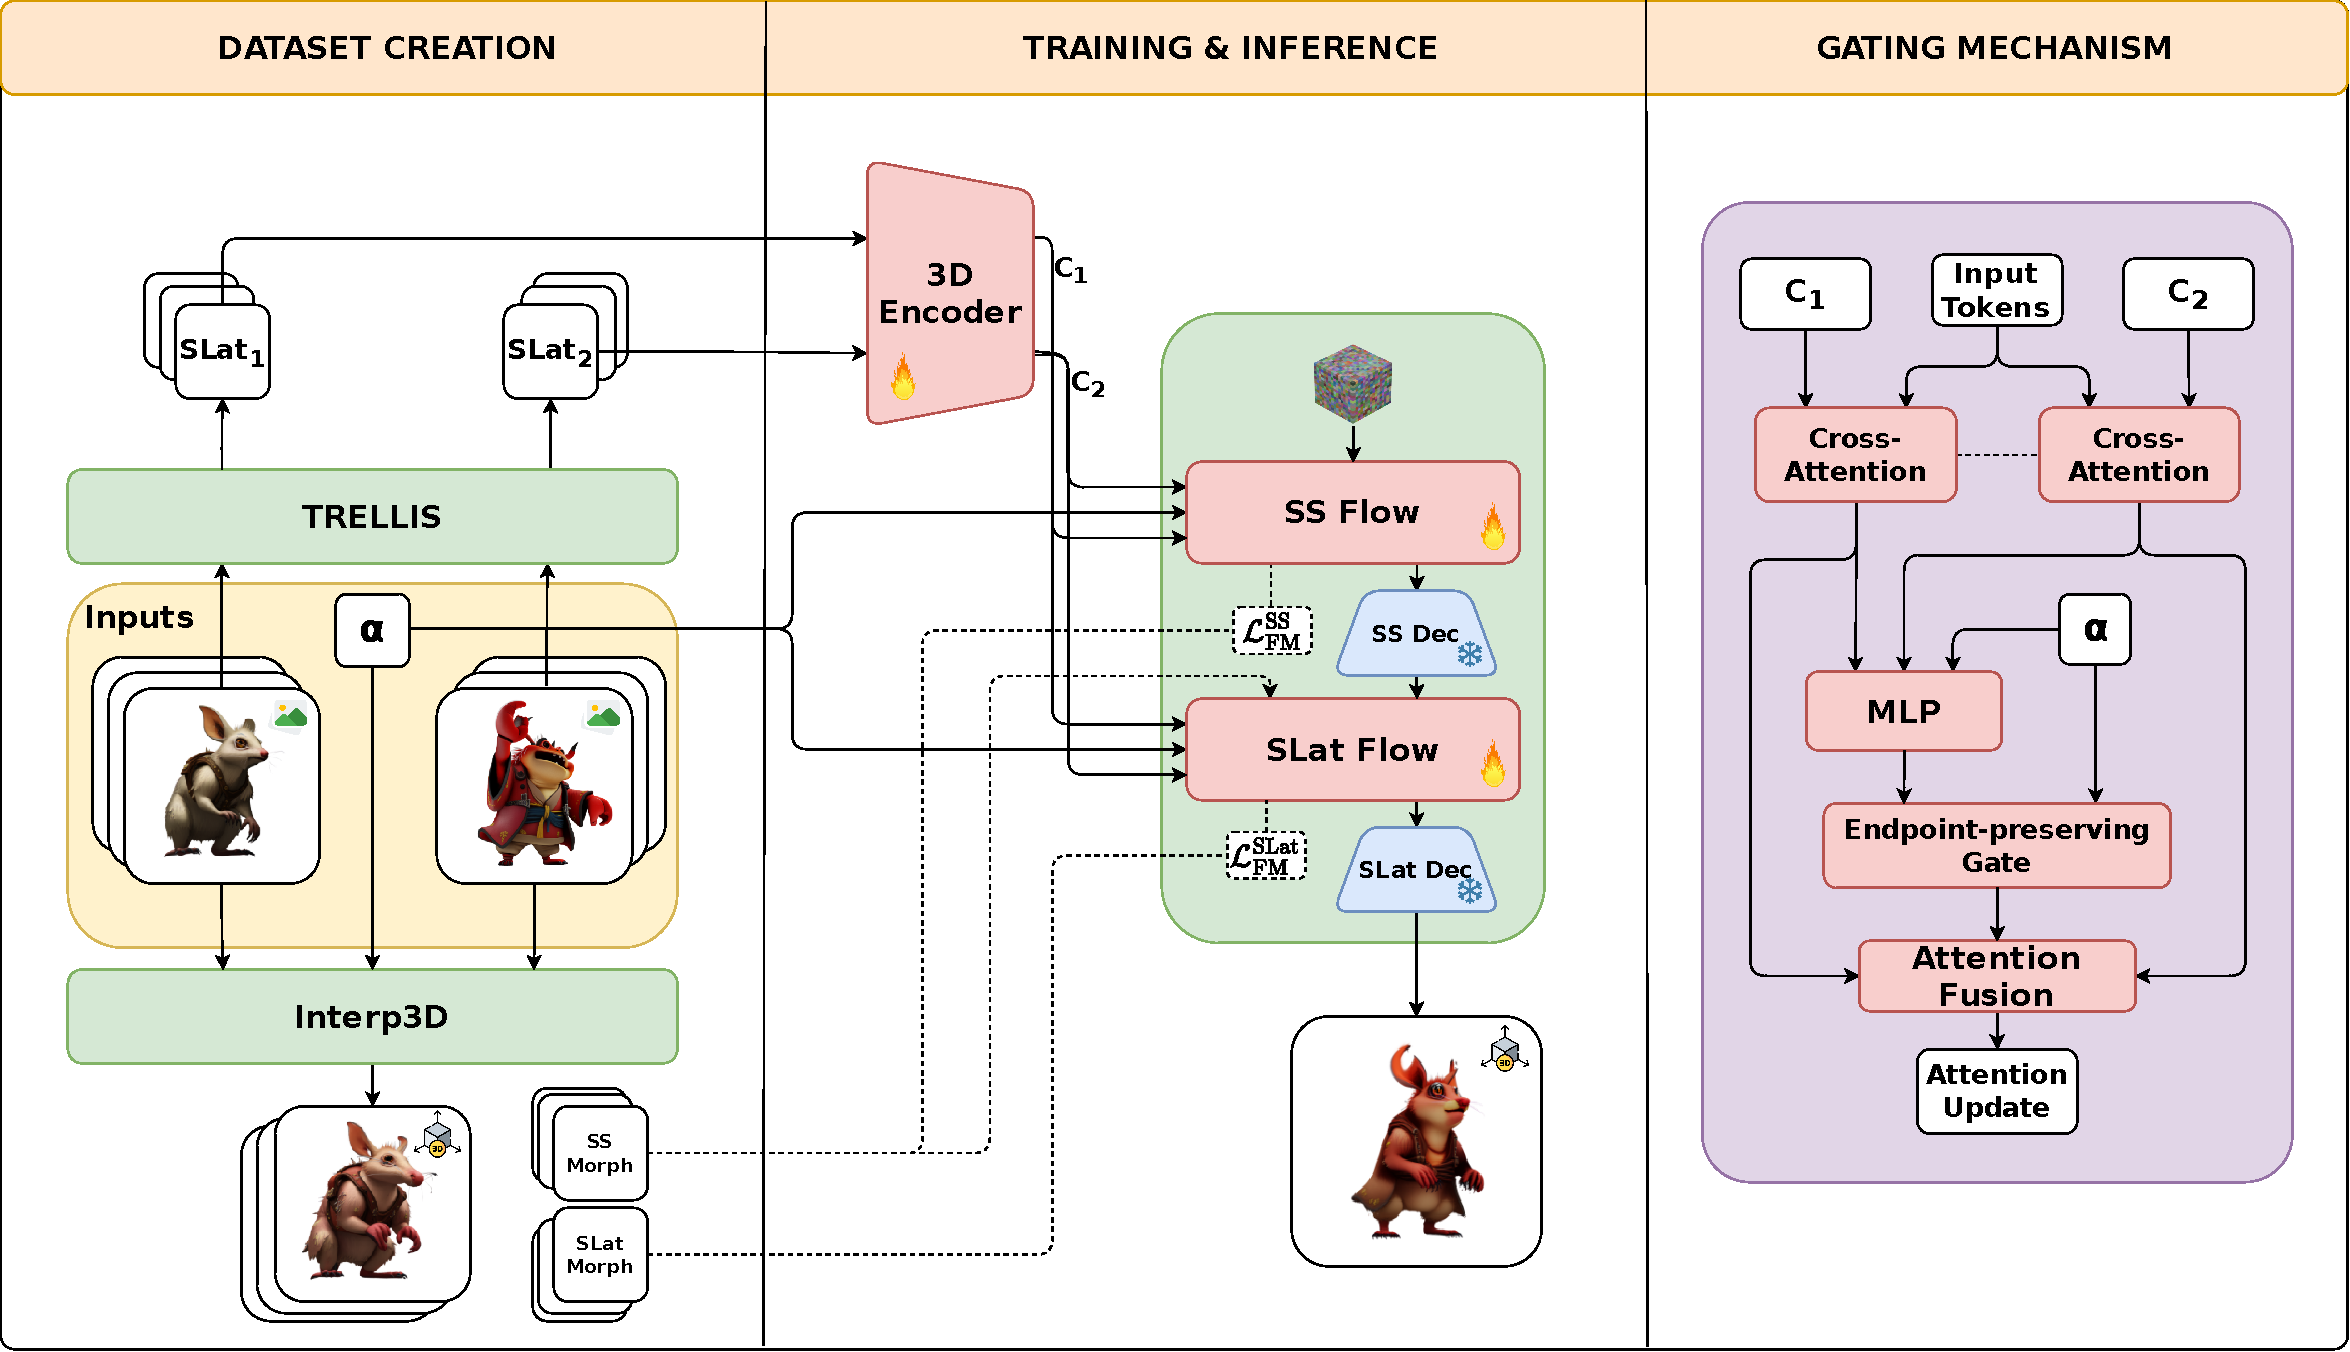
\includegraphics[width=\textwidth]{figures/architecture_overview.pdf}
 \caption{\textbf{Learning textured 3D morphing.} Interp3D produces latent
 targets from source pairs and interpolation coefficients. The student
 encodes each source SLat independently and generates sparse structure and
 structured features. The right panel shows two evaluations of the same
 cross-attention on the source conditions, followed by learned gating.
 Flames mark modules with trainable parameters; snowflakes mark frozen
 decoders. Dashed supervision connections are used during training.}
 \label{fig:architecture}
\end{figure*}

\subsection{Preliminaries}
\label{sec:preliminaries}
%TRELLIS~\cite{xiang2025trellis} is a 3D generation method which represents 3D assets through structured latents (SLat). Instead of encoding an entire object in a single vector, SLat associates local feature vectors with the occupied locations of a sparse 3D grid. The active voxel positions describe the object's spatial support, while the features carried by those positions contain information about its geometry and appearance. This separation makes it possible to model where an object exists in space and what its local structure looks like.
TRELLIS\cite{xiang2025trellis} generates 3D assets conditioned on images or text using structured latents (SLat). In this representation, each active location of a sparse 3D grid carries local features describing geometry and appearance. The representation therefore separates the asset’s spatial support from the information associated with each occupied location.

To generate these latents, TRELLIS uses two successive transformer-based rectified flows~\cite{xiang2025trellis,liu2023rectifiedflow}. First, the sparse-structure (SS) flow predict a latent from which the occupied grid locations are decoded; conditioned on this support, the SLat flow then generates their local features. For image-conditioned generation, DINOv2~\cite{oquab2023dinov2} encodes the input image into visual tokens that condition both flows through cross-attention. The resulting SLat representation can then be decoded into a mesh, 3D Gaussian splats~\cite{kerbl2023gaussians}, or a radiance field~\cite{mildenhall2020nerf}.

Building on this representation, we adapt both the SS and SLat flows within the same morphing framework, adapting them to work with a pair of source 3D assets.

\subsection{Framework}
\subsubsection{Training Dataset Construction}
\label{sec:dataset_construction}
Since ground-truth morphing trajectories are not naturally available, we developed a teacher-student framework, using Interp3D ~\cite{liu2026interp3d} as a teacher to generate the training data for our student model. Because Interp3D is image-conditioned, we start from 12,500 distinct pairs of source images, from which the corresponding 3D assets $S_1,S_2$ are generated. For each pair, we then produce four morphing samples at different interpolation coefficients $\alpha\in[0,1]$, including $\alpha=0$ and $\alpha=1$ to encourage the student to reconstruct the source objects. Finally, we extract the corresponding SS and SLat representations from each generated asset. %, which serve as targets for supervising the two stages of our model. 

Each training example therefore contains the two source SLat representations, an interpolation coefficient, and the teacher-generated SS and SLat latents for that coefficient.%, allowing the student to learn morphing transformations directly in the TRELLIS latent space.

\subsubsection{Architecture}
\label{sec:architecture}
% We define our student model as follows. Using the dataset described in Sec.~\ref{sec:dataset_construction}, we adapt the two generation flows of TRELLIS~\cite{xiang2025trellis} to learn 3D morphing transformations directly from the source representations.

% Given two source assets, the student processes their SLat representations through a 3D encoder $\mathcal E_{3D}$, which extracts spatial information from their coordinates and features. The resulting conditioning tokens are projected into the feature space of the pretrained flow transformers:
To learn morphing from these training examples, our student adapts the two generation flows of TRELLIS~\cite{xiang2025trellis} to use conditions extracted directly from the source 3D assets. Let $z_i$ denote the SLat coordinates and features of asset $S_i$. A shared encoder $\mathcal E_{3D}$ maps $z_i$ to conditioning tokens $c_i$, replacing the image-derived conditions used by the original flows:
\begin{equation}
c_i = \mathcal E_{3D}(S_i),
\qquad i\in{1,2}.
\label{eq}
\end{equation}

\noindent 
so that the student can generate morphs from the source 3D representations.

Each condition contains 4096 tokens arranged on a $16\times16\times16$ grid matching the resolution of the SS representation, with positional embeddings encoding their spatial locations. The 1024-dimensional features match the dimensionality of the DINOv2 embeddings used to condition the pretrained TRELLIS cross-attention layers.

Starting from the pretrained TRELLIS weights, we optimize LoRA adapters~\cite{hu2022lora} together with the 3D encoder and the gate network used in the Gate-Adapted Morphing Cross-Attention (GAMCA). Within each transformer block, a gate network $\mathcal G$ learns to combine the responses of a shared cross-attention module to the two source conditions, as described in Sec.~\ref{sec:attention_gating}.


%Obtaining intermediate ground-truth assets for arbitrary  morphing sequences is inherently difficult: we address this lack of supervision by using Interp3D~\cite{liu2026interp3d} as a training-free teacher. Given a pair of assets and an interpolation coefficient, the teacher produces a morph that serves as pseudo-target for the corresponding student generation, allowing us to train on a collection of transitions. By learning shared morphing patterns across diverse objects, the student can generalize beyond individual teacher predictions, reducing teacher-specific artifacts and producing more coherent transitions. The student architecture is structured as follows: (a) a TRELLIS backbone finetuned using LoRA~\cite{hu2022lora}, (b) a 3D encoder $\mathcal{E}_{3D}$ providing the conditions for both TRELLIS flows and (c) an attention gate $\mathcal{G}$ which learns to combine the assets. During training, the teacher supplies intermediate SS and SLat pseudo-targets for source pairs and interpolation coefficients. These pseudo pairs are then encoded  independently using the encoder $\mathcal{E}_{3D}$ that adapts them to be compatible with TRELLIS conditioning mechanism and produces the encoded representations $c_1$ and $c_2$. Finally, $\mathcal{G}$ combines these representations using the coefficient $\alpha$. As teacher, we selected Interp3D~\cite{liu2026interp3d} as it currently represents the best trade off between generation quality and computational efficiency.

% \subsubsection{Learning from latent pseudo-targets}
% \label{sec:teacher_supervision}
% We train the SS and SLat flows with conditional flow matching~\cite{lipman2022flowmatching}, using the teacher-generated latents as supervision. For either stage, let $z_0$ denote the target latent for a source pair and interpolation coefficient $\alpha$. We sample Gaussian noise $\epsilon\sim\mathcal N(0,I)$ and a noise time $\tau\in[0,1]$, and construct
% \begin{align}
%  z_\tau &=(1-\tau)z_0+\sigma_\tau\epsilon,
%  \label{eq:fm_path}\\
%  \sigma_\tau &=\sigma_{\min}+(1-\sigma_{\min})\tau,\nonumber\\
%  u_\tau &=(1-\sigma_{\min})\epsilon-z_0,
%  \nonumber
% \end{align}
% where $\sigma_{\min}$ is a small positive constant controlling the
% residual noise at the data endpoint. Here, $\tau$ specifies the noise
% level, whereas $\alpha$ specifies the position along the morphing
% sequence. The student learns to predict the target velocity $u_\tau$
% from the perturbed latent and the two source conditions:
% \begin{equation}
%  \mathcal L_{\mathrm{FM}}=
%  \mathbb E\!\left[
%  \left\|v_\theta(z_\tau,\tau;c_1,c_2,\alpha)-u_\tau\right\|_2^2
%  \right].
%  \label{eq:flow_matching}
% \end{equation}
% The expectation is over training examples, noise, and noise times.
% To encourage consistency with respect to source ordering, we also
% swap the two sources and replace $\alpha$ with $1-\alpha$, retaining
% the same teacher-generated target.

% Interp3D~\cite{liu2026interp3d} supplies intermediate SS and SLat
% pseudo-targets for source pairs and interpolation coefficients.
% The student retains both TRELLIS flows but conditions them directly on
% the source assets. An asset encoder processes the features and coordinates
% of each source SLat independently, producing $c_1,c_2$.
% LoRA~\cite{hu2022lora} adapts the pretrained flow parameters, while the
% source encoder and attention gate learn to combine the assets.

% In order to finetune our student, conditional flow matching~\cite{lipman2022flowmatching} is used to train each flow against its teacher latents. Let $z_0$ be a target, $\epsilon$ Gaussian noise, $\tau$ the noise timestep and $\sigma_{\min}$ is a small positive hyperparameter controlling the residual noise at the data endpoint. The training path and target velocity are
% \begin{align}
% z_\tau &=(1-\tau)z_0+
%       [\sigma_{\min}+(1-\sigma_{\min})\tau]\epsilon,\\
% u_\tau &=(1-\sigma_{\min})\epsilon-z_0,
% \end{align}
% with objective
% \begin{equation}
% \mathcal L_{\mathrm{FM}}=
% \mathbb E\|v_\theta(z_\tau,\tau;c_1,c_2,\alpha)-u_\tau\|_2^2.
% \end{equation}
% Sampling integrates the learned field from noise toward the latent data. To enforce consistency across source orderings, each training example is augmented by swapping the two source assets and replacing $\alpha$ with $1-\alpha$, while retaining the same teacher-generated target.

\subsubsection{Gate-Adapted Morphing Cross-Attention}
\label{sec:attention_gating}
GAMCA combines the responses of the cross-attention module to the two source conditions through a learnable gate. While the interpolation coefficient $\alpha$ controls the overall balance between the sources, the gate adjusts their relative contributions across latent tokens and feature channels, allowing different parts of the morph to combine source features differently. The same mechanism is applied in both the SS and SLat generation stages, where each transformer block processes latent tokens $x\in\mathbb R^{N\times d}$ with $d=1024$.

The SS flow operates on a fixed set of $N=4096$ tokens, whereas the SLat flow processes a variable number of active tokens, determined by the asset's spatial support at the transformer resolution.
In either case, the current latent are provided to the cross-attention operator, denoted by $\operatorname{CA}$, which is evaluated separately on the two source conditions:
% First of all, two evaluations of the cross-attention module produce source-specific responses:
\begin{equation}
 h_1=CA(x,c_1),\qquad h_2=CA(x,c_2),
\end{equation}
The resulting responses $h1, h2$ are then combined using weights that adapt to their features and to the interpolation coefficient $\alpha$:
\begin{equation}
 \begin{aligned}
  \delta &=\mathcal G(h_1,h_2,\alpha),\\
  g &=(1-\alpha)+\alpha(1-\alpha)\tanh(\delta),\\
  x &\leftarrow x+(1-g)\odot h_1+g\odot h_2,
 \end{aligned}
 \label{eq:attention_gate}
\end{equation}
where $\mathcal G$ is an MLP that predicts the residual adjustment $\delta$, while $g$ contains the resulting mixing weights. Both $\delta$ and $g$ have the same dimensions as $x$, and $\odot$ denotes elementwise multiplication.

We initialize $\mathcal G$ to output zero, so the fusion initially reduces to $\alpha h_1+(1-\alpha)h_2$. As training progresses, the network learns to adjust this mixture according to the source responses and the current generation state. Because the adjustment is multiplied by $\alpha(1-\alpha)$, it vanishes at $\alpha=0$ and $\alpha=1$, leaving only $h_2$ or $h_1$, respectively. At these coefficient values, generation therefore uses only the corresponding source condition, while reconstruction is learned from the teacher targets.
% In order to define a fusion mechanism that can both perform the morphing while maintaining exact endpoints reconstruction we defined an attention gating mechanism which is shared in both generation flows.

% Specifically, within each attention block, the current tokens $x$ attend independently to the two source conditions through cross-attention:
% \begin{equation}
%  h_1=A_\theta(x,c_1),\qquad h_2=A_\theta(x,c_2).
% \end{equation}

% The two attention responses are then fused through a token- and channel-wise gate:
% \[
% \begin{aligned}
% \delta &= \operatorname{MLP}(h_1,h_2,\alpha),\\
% g &= (1-\alpha)+\alpha(1-\alpha)\tanh(\delta),\\
% x &\leftarrow x+(1-g)\odot h_1+g\odot h_2.
% \end{aligned}
% \]

% The MLP is initialized to produce zero outputs, so the fusion initially reduces to \(\alpha h_1+(1-\alpha)h_2\). During training, the learned residual adaptively adjusts the contributions of each source, while the factor \(\alpha(1-\alpha)\) ensures that the correction vanishes at both endpoints, preserving single-source conditioning.
\subsubsection{Training and generative-prior regularization}
\label{sec:teacher_supervision}
\label{sec:generative_prior}

We train the SS and SLat flows using the standard conditional flow-matching objective~\cite{lipman2022flowmatching}, denoted by $\mathcal L_{\mathrm{FM}}$, with the teacher-generated latents as targets. Each target is associated with a source pair and an interpolation coefficient $\alpha$. During training, we also swap the sources and replace $\alpha$ with $1-\alpha$, keeping the target unchanged to encourage consistency with respect to source ordering.

To complement this supervision, we use a generative prior that acts on samples produced by the student. For each stage, the prior is provided by a separate copy of the original image-conditioned TRELLIS flow, kept frozen throughout training. It uses the source images $I_1$ and $I_2$ from which the training assets $S_1$ and $S_2$ were obtained.

We first generate a latent $\hat z$ by running the student's complete sampling procedure from Gaussian noise, conditioned on $c_1$, $c_2$, and $\alpha$. Once generation is complete, we perturb $\hat z$ with fresh Gaussian noise at a sampled noise level, following the TRELLIS noise schedule. The frozen flow then evaluates this same perturbed sample twice, using the DINOv2 embedding~\cite{oquab2023dinov2} of $I_1$ in one evaluation and that of $I_2$ in the other. Each predicted velocity is converted into an estimate of the clean latent under the corresponding source-image condition. To obtain the regression targets $\tilde z_1$ and $\tilde z_2$, we adjust $\hat z$ toward each estimate. We limit the size of each adjustment so that the targets remain close to the student's generated sample.

The prior loss encourages the student output to approach these targets, with $\alpha$ determining the contribution of each source:
\begin{equation}
 \mathcal L_{\mathrm{prior}}=
 \mathbb E\!\left[
 \frac{\alpha}{2}\operatorname{MSE}(\hat z,\tilde z_1)
 +\frac{1-\alpha}{2}\operatorname{MSE}(\hat z,\tilde z_2)
 \right].
 \label{eq:prior}
\end{equation}
At $\alpha=1$, only the term associated with $S_1$ remains, while at $\alpha=0$ only the term associated with $S_2$ remains. The targets are treated as fixed during backpropagation: gradients pass through $\hat z$ to update the student's trainable modules, without differentiating through the target computation. The original TRELLIS flow remains frozen.

The overall objective combines teacher supervision and generative regularization:
\begin{equation}
 \mathcal L=\mathcal L_{\mathrm{FM}}
 +\lambda_{\mathrm{prior}}\mathcal L_{\mathrm{prior}},
\end{equation}
where $\lambda_{\mathrm{prior}}$ controls the contribution of the prior. The frozen flows and source images are needed only during training.

Algorithm~\ref{alg:generative_prior} summarizes the training
procedure, applied to either the SS or SLat flow.

\begin{algorithm}[t]
\caption{Training with a frozen generative prior}
\label{alg:generative_prior}
\small
\begin{algorithmic}[1]
\Require Source conditions $c_1,c_2$, images $I_1,I_2$,
coefficient $\alpha$
\Require Frozen TRELLIS flow $T$, teacher-supervised loss
$\mathcal L_{\mathrm{FM}}$, prior weight $\lambda_{\mathrm{prior}}$

\Statex \textit{Generate a student sample.}
\State Generate $\hat z$ by completing student sampling from
Gaussian noise, conditioned on $(c_1,c_2,\alpha)$

\Statex \textit{Build fixed targets without gradient tracking.}
\State Sample a noise level $\tau$
\State Perturb $\hat z$ with fresh Gaussian noise at level $\tau$,
using the TRELLIS noise schedule, to obtain $\hat z_\tau$
\For{$i\in\{1,2\}$}
    \State $v_i \gets
    T(\hat z_\tau,\tau;\operatorname{DINOv2}(I_i))$
    \State Convert $v_i$ into a clean-latent estimate $\bar z_i$
    \State $\Delta_i \gets \bar z_i-\hat z$
    \If{the magnitude of $\Delta_i$ exceeds its limit}
        \State Reduce the magnitude of $\Delta_i$,
        keeping its direction
    \EndIf
    \State $\tilde z_i \gets \hat z+\Delta_i$
\EndFor

\Statex \textit{Compute the loss and update the student.}
\State $\mathcal L_i \gets
\tfrac12\operatorname{MSE}(\hat z,\tilde z_i)$,
for $i\in\{1,2\}$
\State $\mathcal L_{\mathrm{prior}} \gets
\alpha\mathcal L_1+(1-\alpha)\mathcal L_2$
\State $\mathcal L \gets
\mathcal L_{\mathrm{FM}}
+\lambda_{\mathrm{prior}}\mathcal L_{\mathrm{prior}}$
\State Update the student's trainable parameters using
$\mathcal L$, treating $\tilde z_1,\tilde z_2$ as fixed targets
\end{algorithmic}
\end{algorithm}

% \subsubsection{Generative-prior regularization via frozen flow predictions}
% \label{sec:generative_prior}

% Teacher supervision provides examples of transitions, but it does not
% directly assess the samples generated by the student. We therefore add a
% generative prior that acts on the student's own outputs during training.

% Starting from Gaussian noise $\eta$, we integrate the student flow under
% the two source conditions and the interpolation coefficient, obtaining
% $\hat z=G_\theta(\eta;c_1,c_2,\alpha)$. 

% Then, we perturb the generated latent with fresh Gaussian noise $\epsilon$ at
% a sampled noise time $\tau$:
% \begin{equation}
%  z_\tau=(1-\tau)\hat z+\sigma_\tau\epsilon,
%  \qquad
%  \sigma_\tau=\sigma_{\min}+(1-\sigma_{\min})\tau.
% \end{equation}
% The frozen, image-conditioned TRELLIS flow evaluates this same perturbed
% sample twice, using the DINOv2 embedding~\cite{oquab2023dinov2} of $I_1$
% in one evaluation and that of $I_2$ in the other. Each predicted velocity
% provides an estimate of the clean latent under its source-image
% condition. A bounded local correction derived from that estimate defines
% a nearby regression target $\tilde z_i$ for the student sample.
% The two targets therefore express how the same generated asset should
% change under the two source conditions.

% The source-conditioned prior loss combines these regression errors:
% \begin{equation}
%  \mathcal L_{\mathrm{prior}}=
%  \mathbb E\!\left[
%  \frac{\alpha}{2}\operatorname{MSE}(\hat z,\tilde z_1)
%  +\frac{1-\alpha}{2}\operatorname{MSE}(\hat z,\tilde z_2)
%  \right].
%  \label{eq:prior}
% \end{equation}
% \noindent, with the interpolation coefficient $\alpha$ setting
% the relative influence of the two source-conditioned corrections. At
% $\alpha=1$ only the first term remains, and at $\alpha=0$ only the
% second remains. TRELLIS receives one source image at a time; the
% interpolation coefficient combines the two losses rather than the image
% embeddings.
% The student's trainable modules are updated, while TRELLIS
% remains frozen.

% The complete training objective is
% \begin{equation}
%  \mathcal L=\mathcal L_{\mathrm{FM}}
%  +\lambda_{\mathrm{prior}}\mathcal L_{\mathrm{prior}},
% \end{equation}
% where $\lambda_{\mathrm{prior}}$ controls the influence of the
% generative feedback relative to teacher supervision.


